\section{Ablation studies}
\label{sec:ablation}


\subsection{Effect of example method} 
\label{sec:ablation-example}
An advantage of SchemaRAG is its openness to the use of any extra annotated data. When a set of annotated examples $A$ is available, it could be incorporated in three ways: i) as example embeddings that drive the schema reduction process (``to-schema''), ii) as in-context learning material that is injected into the prompt (``to-prompt''), or iii) both (``to-both''). We examine the effect of these example methods on the extraction performance of SchemaRAG on the Nursing dataset, breaking down by hospital (Figure \ref{fig:exampleablation}).


\begin{figure}[t]
    \centering 
    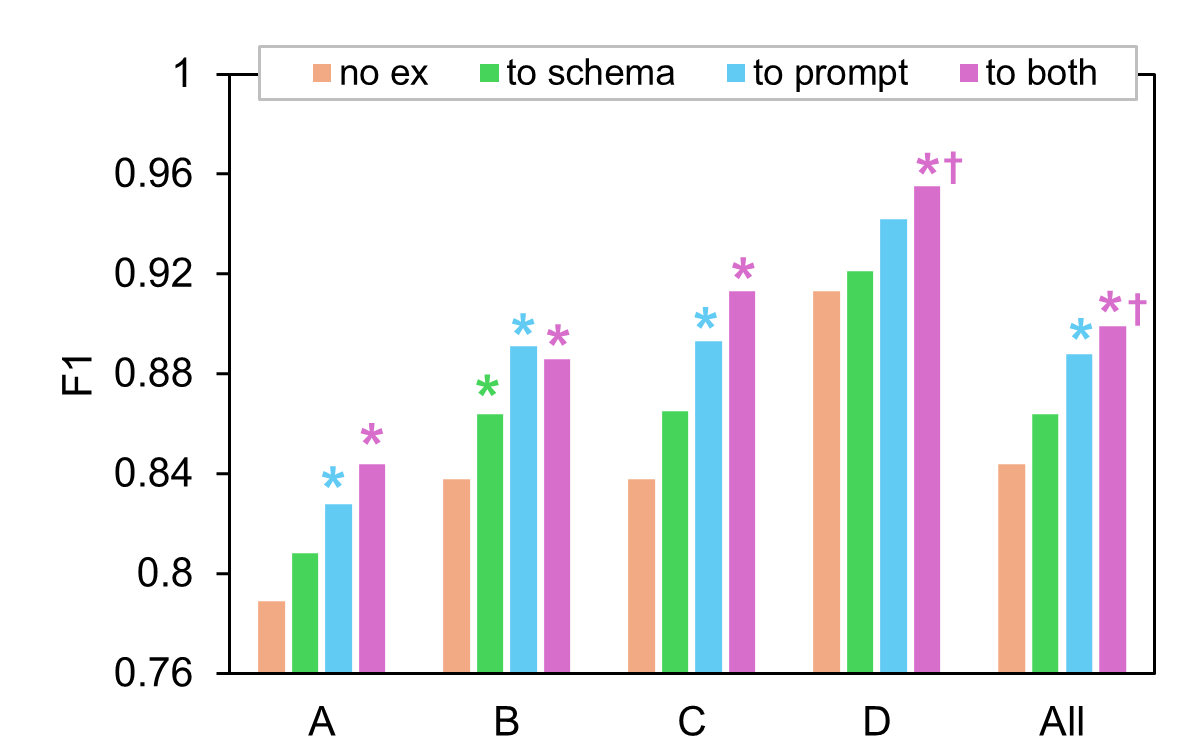
\includegraphics[width=\linewidth]{img/exampleablation3.png}
    \caption{Effect of example use method on SchemaRAG F\textsubscript{1} on the Nursing dataset. * indicates significance over the no-example baseline, and \textsuperscript{\textdagger} over the ``to-prompt'' method, at $p <$ 0.01.}
    \label{fig:exampleablation}
\end{figure}



Across all four hospitals, the ``to-both'' method significantly improves extraction accuracy over the no-example baseline. This demonstrates that incorporating guidance from examples at both the retrieval and inference stages is effective across different schema structures.

The gain from the ``to-schema'' method alone is not statistically significant. In contrast, the ``to-prompt'' method yields a statistically significant improvement alone, indicating that few-shot supervision at inference time plays a central role in guiding accurate extraction. The performance of the ``to-both'' method also significantly exceeds that of the ``to-prompt'' method.
This suggests that inclusion of example embeddings in retrieval, in addition to in-prompt example text,
yields complementary information that helps improve alignment between the reduced schema and relevant prompt content.

\subsection{Effect of row and example embeddings} 
We examine how row embeddings and example embeddings, used independently and together during the retrieval stage, affect extraction performance on the Nursing dataset. 
All pairwise differences between conditions are statistically significant (Table~\ref{tab:embeddingablation}).

Using only example embeddings yields the lowest performance. This can be partly attributed to the fact that each per-hospital example set does not cover all rows present in the per-hospital test set. Some test rows have no corresponding examples (see Figure~\ref{fig:coverage}), placing a fundamental limit on row recall. Additionally, the example set contains schema rows that are not part of the test set, which introduces noise. By
contrast, row-level embeddings provide complete coverage and ensure that all schema entries are potentially retrievable. 

The superior performance of combining both embeddings highlights their complementary nature: row embeddings offer broad coverage, while example embeddings provide context-rich signals when available.

\subsection{Effect of segmentation} 
We evaluate the role of segmentation in SchemaRAG by comparing three conditions: i) no segmentation at all, ii) segmentation used only for scoping the RAG process (with the full transcript and the union over all segments' resulting reduced schemas as the $S_\kappa$  provided to a single LLM call at extraction), iii) and full segmentation used both in RAG and prompt construction over per-segment extraction calls (see Table~\ref{tab:segablation}). 

On the Nursing dataset, both segmentation conditions significantly outperform the no-segmentation baseline. On the Amazon dataset, segmentation for scoping RAG significantly outperforms no segmentation, though its advantage over full segmentation used both in RAG and prompt construction is not statistically significant. These results suggest that segmentation benefits SchemaRAG primarily by guiding schema selection during the retrieval phase. Additional gains from segment-level extraction itself
depend on the domain and dataset characteristics.

\begin{table}
    \centering
    \caption{Effect of row and example embedding availability in SchemaRAG retrieval ($k=60$) on average per-transcript extraction performance on the Nursing dataset. All pairwise differences are statistically significant, indicated by \textsuperscript{\textdagger} ($p < 0.001$).}
    \label{tab:embeddingablation}
    \begin{tabular}{lll}
        \toprule
        \textbf{Row} & \textbf{Example} & \textbf{macro-F\textsubscript{1}} \\
        \midrule 
        yes & no & 0.888\textsuperscript{\textdagger} \\
        no & yes & 0.798\textsuperscript{\textdagger} \\
        yes & yes & \textbf{0.899}\textsuperscript{\textdagger} \\
        \bottomrule
    \end{tabular}
\end{table}

\begin{table}
    \centering
    \caption{Effect of segmentation scope on extraction performance of SchemaRAG. Statistical significance vs. no-segmentation SchemaRAG baseline is indicated by 
    * ($p <$ 0.05) and
    \textsuperscript{\textdagger} ($p < 0.001$).}
    \label{tab:segablation}
    \begin{tabular}{lll}
        \toprule
        \textbf{Segmentation scope} & \multicolumn{2}{c}{\textbf{macro-F\textsubscript{1}}} \\
        & Nursing & Amazon \\
        \midrule 
        Baseline & 0.774 & 0.484\\
        \midrule 
        RAG-only & 0.898\textsuperscript{\textdagger} & \textbf{0.554}* \\
        RAG + prompt & \textbf{0.899}\textsuperscript{\textdagger} & 0.515 \\
        \bottomrule
    \end{tabular}
\end{table}


\subsection{Effect of \boldmath$k$} 
We examine the effect of the hyperparameter $k$ on the extraction performance of SchemaRAG on the Nursing dataset. $k$ is the number of embeddings consulted during the schema reduction process and roughly correlates with $\kappa$, the final number of rows in the reduced schema. We vary $k$ to produce reduced schemas of size $\kappa$ between 1 and 1100 with and without segmentation, and with and without examples, running each condition only once (Figure \ref{fig:varyk}). 

In general, increasing $k$ improves performance to a point, as the relevant rows appear in the reduced schema; but performance saturates and declines as $k$ increases, as the reduced schema becomes too large and the LLM is unable to focus on the relevant rows. This effect holds over all segmentation and example conditions, though using segmentation and examples shift the optimal $k$ to a lower value.

\begin{figure}[!t]
    \centering
    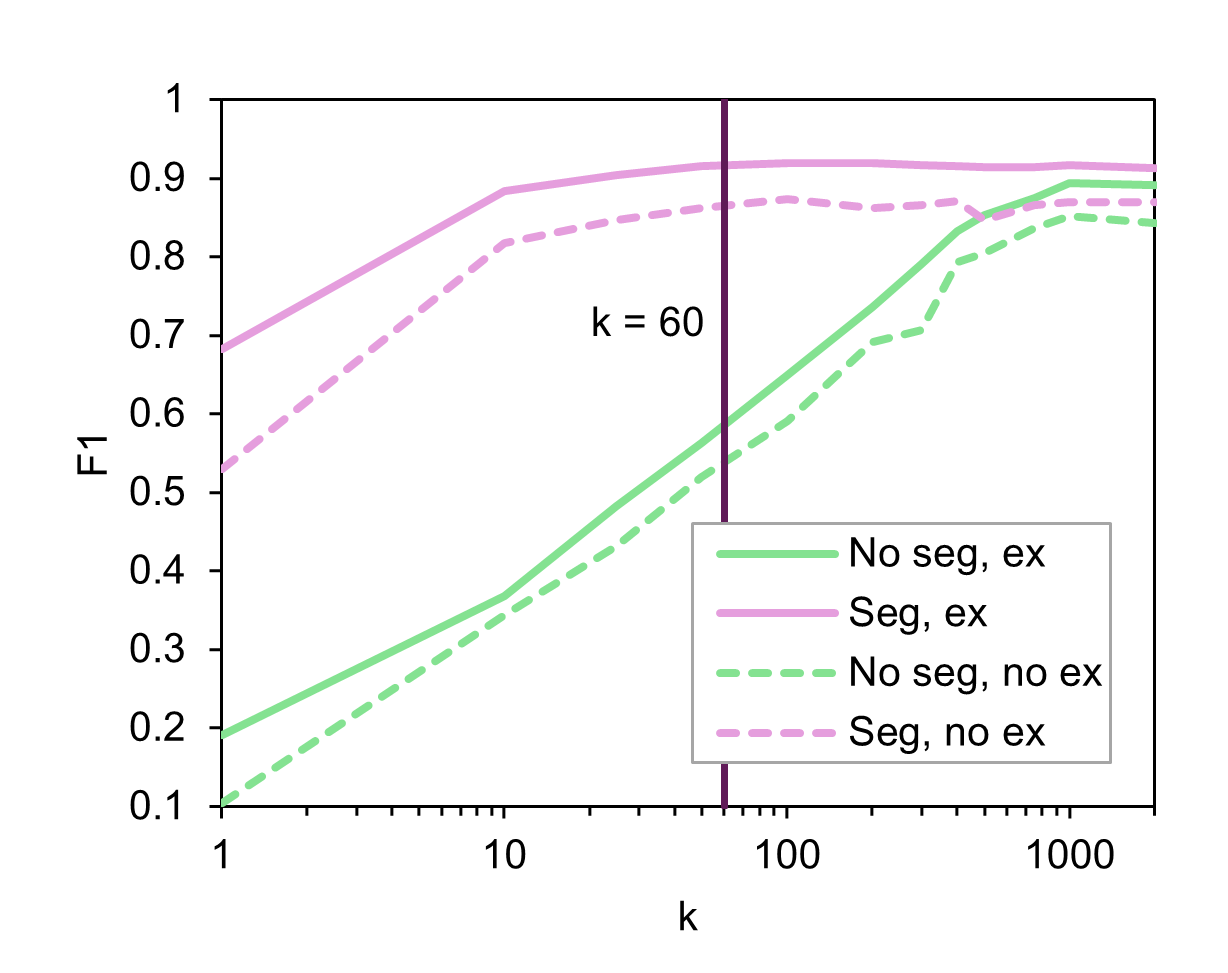
\includegraphics[width=\linewidth]{img/varyk_2.png}
    \caption{Effect of $k$ on SchemaRAG F\textsubscript{1} on Nursing.}
    \label{fig:varyk}
\end{figure}

\begin{table}[t]
    \centering
    \caption{Comparison of Precision and Recall between the Full-schema baseline and SchemaRAG at various levels (@$k$).}
    \label{tab:results_comparison}
    \begin{tabular}{@{}lccccc@{}}
        \toprule
        \textbf{Method} & \textbf{@\boldmath$k$} & \textbf{Precision} & \textbf{Recall} \\ \midrule
        Full-schema + seg. & 1  & 0.724 & 0.431 \\
                                   & 5  & 0.275 & 0.749 \\
                                   & 10 & 0.161 & 0.857 \\
                                   & 30 & 0.060 & 0.948 \\
                                   & 60 & 0.031 & 0.981 \\ 
        \midrule
        \textbf{SchemaRAG}         & 1  & 0.837 & 0.503 \\
                                   & 5  & 0.288 & 0.800 \\
                                   & 10 & 0.163 & 0.886 \\
                                   & 30 & 0.060 & 0.959 \\
                                   & 60 & 0.031 & 0.991 \\
        \bottomrule
    \end{tabular}
\end{table}


\subsection{Retrieval upper bound via Precision/ Recall@\boldmath$k$} 
We compare SchemaRAG to a full-schema baseline that uses segmentation to eliminate the effect of segmentation on top-$k$ counting. Each segment of a transcript yields its own SchemaRAG-retrieved set of rows; we take the top $k$ of each segment, then combine these and compare to the gold-standard annotations for the entire transcript.

SchemaRAG achieves consistently higher recall@$k$ than the full-schema+segmentation baseline at equivalent k values (Table~\ref{tab:results_comparison}). This suggests that SchemaRAG yields more of the annotated rows than the naïve baseline and approaches the upper bound of retrieval faster with increasing $k$.

Similarly, SchemaRAG exhibits higher precision@$k$ at low $k$  (Table~\ref{tab:results_comparison}), suggesting that the annotated rows it finds are more densely packed near the top of the retrieval. (At high $k$, the baseline and SchemaRAG have similar precisions because there are more cases of fewer than $k$ annotated rows over each transcript).
